% This example is meant to be compiled with lualatex or xelatex
% The theme itself also supports pdflatex
\PassOptionsToPackage{unicode}{hyperref}
\documentclass[aspectratio=1610, 12pt]{beamer}

% Warning, if another latex run is needed
% \usepackage[aux]{rerunfilecheck}

% just list chapters and sections in the toc, not subsections or smaller
\setcounter{tocdepth}{1}

%------------------------------------------------------------------------------
%------------------------------ Fonts, Unicode, Language ----------------------
%------------------------------------------------------------------------------
\usepackage{fontspec}
\defaultfontfeatures{Ligatures=TeX}  % -- becomes en-dash etc.

% german language
\usepackage{polyglossia}
\setdefaultlanguage{german}

% for english abstract and english titles in the toc
\setotherlanguages{english}

% intelligent quotation marks, language and nesting sensitive
\usepackage[autostyle]{csquotes}

% microtypographical features, makes the text look nicer on the small scale
\usepackage{microtype}

%------------------------------------------------------------------------------
%------------------------ Math Packages and settings --------------------------
%------------------------------------------------------------------------------

\usepackage{amsmath}
\usepackage{amssymb}
\usepackage{mathtools}
\usepackage{bbold}

% Enable Unicode-Math and follow the ISO-Standards for typesetting math
\usepackage[
  math-style=ISO,
  bold-style=ISO,
  sans-style=italic,
  nabla=upright,
  partial=upright,
]{unicode-math}
\setmathfont{Latin Modern Math}

% nice, small fracs for the text with \sfrac{}{}
\usepackage{xfrac}


%------------------------------------------------------------------------------
%---------------------------- Numbers and Units -------------------------------
%------------------------------------------------------------------------------

\usepackage[
  locale=DE,
  separate-uncertainty=true,
  per-mode=symbol-or-fraction,
]{siunitx}
\sisetup{math-micro=\text{µ},text-micro=µ}
% \sisetup{tophrase={{ to }}}
%------------------------------------------------------------------------------
%-------------------------------- tables  -------------------------------------
%------------------------------------------------------------------------------

\usepackage{booktabs}       % \toprule, \midrule, \bottomrule, etc

%------------------------------------------------------------------------------
%-------------------------------- graphics -------------------------------------
%------------------------------------------------------------------------------

\usepackage{graphicx}
%\usepackage{rotating}
\usepackage{grffile}
\usepackage{tikz}
\usepackage{circuitikz}
\usepackage{tikz-feynman}
\usepackage{subcaption}

% allow figures to be placed in the running text by default:
\usepackage{scrhack}
\usepackage{float}
\floatplacement{figure}{htbp}
\floatplacement{table}{htbp}

% keep figures and tables in the section
\usepackage[section, below]{placeins}

% smileys
\usepackage{MnSymbol,wasysym}

%------------------------------------------------------------------------------
%---------------------- customize list environments ---------------------------
%------------------------------------------------------------------------------

\usepackage{enumitem}
\usepackage{listings}
\usepackage{hepunits}

\usepackage{pdfpages}
%------------------------------------------------------------------------------
%------------------------------ Bibliographie ---------------------------------
%------------------------------------------------------------------------------

\usepackage[
  backend=biber,   % use modern biber backend
  autolang=hyphen, % load hyphenation rules for if language of bibentry is not
                   % german, has to be loaded with \setotherlanguages
                   % in the references.bib use langid={en} for english sources
]{biblatex}
\addbibresource{references.bib}  % the bib file to use
\DefineBibliographyStrings{german}{andothers = {{et\,al\adddot}}}  % replace u.a. with et al.


% Load packages you need here
% \usepackage{polyglossia}
% \setmainlanguage{german}

\usepackage{csquotes}


% \usepackage{amsmath}
% \usepackage{amssymb}
% \usepackage{mathtools}

\usepackage{hyperref}
\usepackage{bookmark}

% load the theme after all packages

\usetheme[
  showtotalframes, % show total number of frames in the footline
]{tudo}

% Put settings here, like
\unimathsetup{
  math-style=ISO,
  bold-style=ISO,
  nabla=upright,
  partial=upright,
  mathrm=sym,
}

% \setbeamertemplate{itemize item}{\scriptsize$\blacktriangleright$}
% \setbeamertemplate{itemize subitem}{\scriptsize$\blacktriangleright$}

%Titel:
\title{Stability measurement for SciFi modules alignment}
%\subtitle{tuning of uncertainties}
%Autor
\author[N.Breer]{Nils Breer}
%Lehrstuhl/Fakultät
\institute{TU Dortmund, AG Albrecht}
%\titlegraphic{\includegraphics[width=0.3\textwidth]{content/Bilder/interferenz.jpg}}
% \date{12.05.2023}

\begin{document}
\maketitle

\begin{frame}\frametitle{Dataset and motivation}
  \begin{columns}
    \begin{column}[c]{0.48\textwidth}
      \begin{itemize}
        \setlength\itemsep{0em}
        \item $\bullet$\, \href{https://twiki.cern.ch/twiki/bin/viewauth/LHCbInternal/CommissioningData2022}{Dataset} contains magUp and magDown sample from 2022 labeled as "good" from EMTF 
        \item $\bullet$\, Good: > 90\% of datalinks are good
        \item $\bullet$\, runs from fills: 8489, 8491, 8496
        \item $\bullet$\, Using V10 Alignment from tag
      \end{itemize}
    \end{column}
    \begin{column}[c]{0.48\textwidth}
      Motivation:
      \begin{itemize}
        \setlength\itemsep{0em}
        \item $\bullet$\, check how much the SciFi moves between runs
        \begin{itemize}
          \item $\bullet$\, compare the position of adjecent runs in ascending order from my list of runs
          \item list of chosen runs: 255949, 256030, 256145, 256159, 256163, 256272, 256278, 256290
        \end{itemize}
        \item $\bullet$\, check where the half modules are in their local frame
      \end{itemize}
    \end{column}
  \end{columns}
\end{frame}

\begin{frame}\frametitle{Module Positions in local half module frame}
  \begin{columns}
    \begin{column}[c]{0.48\textwidth}
      \begin{itemize}
        \item $\bullet$\, Runs 255949 + 256030 were from fill 8489
        \item $\bullet$\, Optimal fine timing implemented in 256145 (afterwards)
        \item $\bullet$\, Positions of other runs compatible (reminder: MU and MD mixed)
      \end{itemize}
    \end{column}
    \begin{column}[c]{0.48\textwidth}
      \begin{figure}
        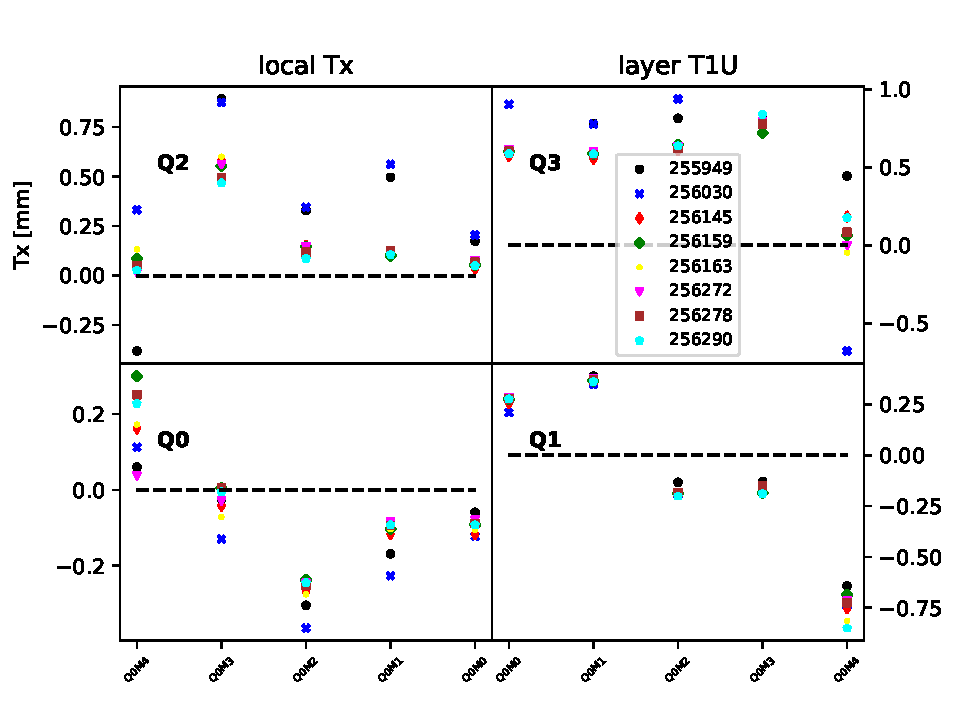
\includegraphics[width=0.9\textwidth]{plots/plain_data/raw_data_T1U_Tx.pdf}
      \end{figure}
    \end{column}
  \end{columns}
\end{frame}

\begin{frame}\frametitle{Module positions: magUp and magDown in x-direction}
  \begin{columns}
    \begin{column}[c]{0.48\textwidth}
      \begin{itemize}
        \item $\bullet$\, magUp and magDown runs are compatible respectively
        \item $\bullet$\, Module positions did not change much except for the black and blue runs
      \end{itemize}
      \begin{figure}
        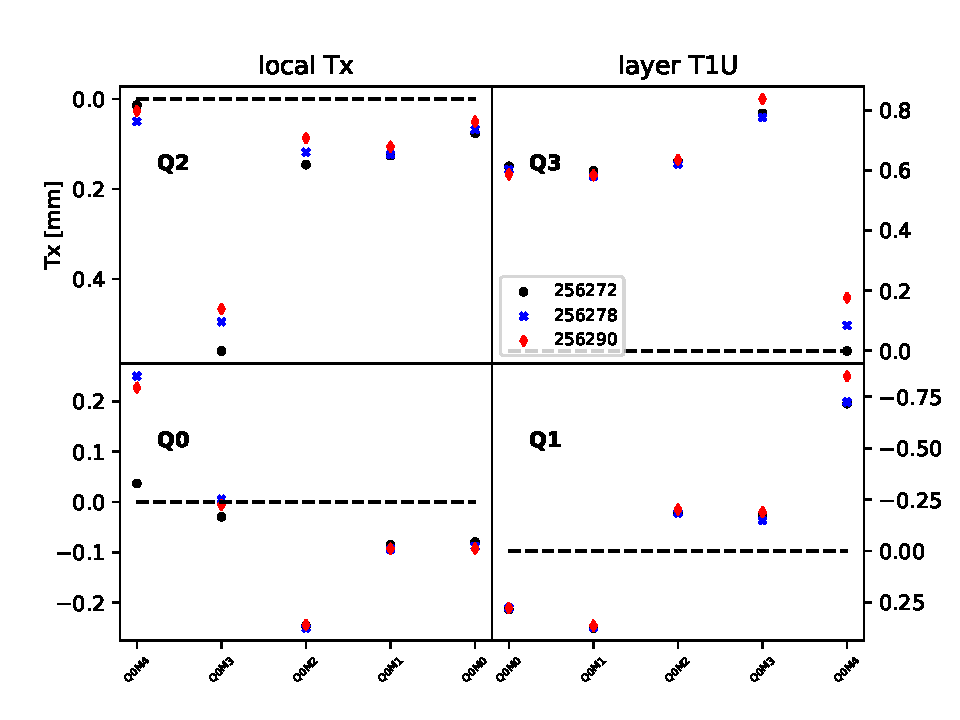
\includegraphics[width=0.7\textwidth]{plots/plain_data/raw_MU_T1U_Tx.pdf}
      \end{figure}
    \end{column}
    \begin{column}[c]{0.48\textwidth}
      \begin{figure}
        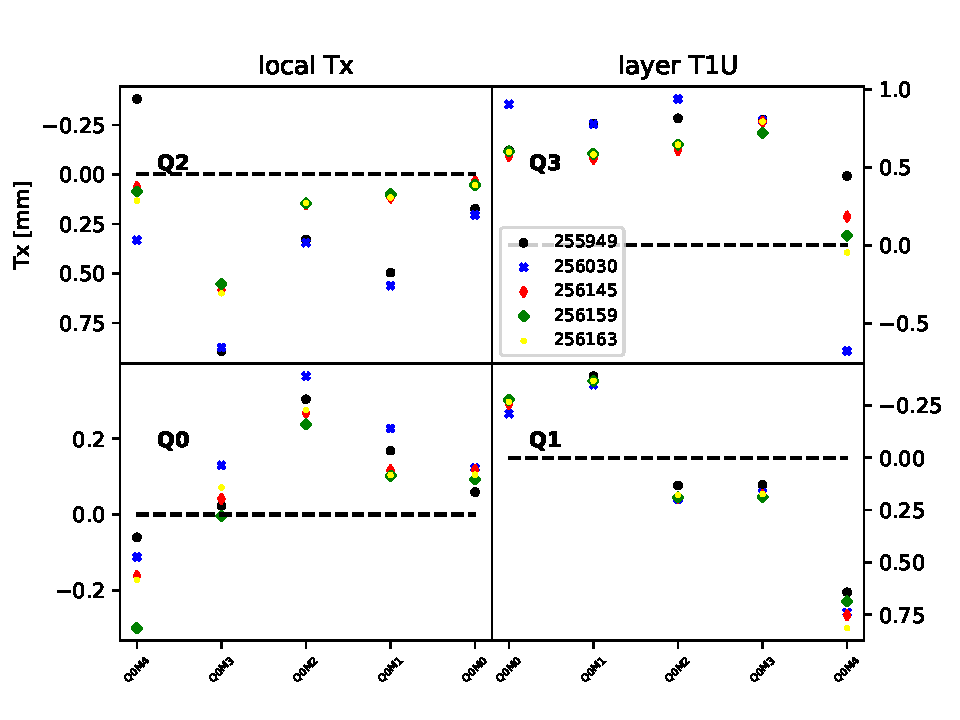
\includegraphics[width=0.7\textwidth]{plots/plain_data/raw_MD_T1U_Tx.pdf}
      \end{figure}
    \end{column}
  \end{columns}
\end{frame}

\begin{frame}\frametitle{Difference between runs: Tx}
  \begin{columns}
    \begin{column}[c]{0.48\textwidth}
      \begin{itemize}
        \item $\bullet$\, Outer module (M4) always worse than the inner modules (a lot less events)
        \item $\bullet$\, Largest movement: T1VQ1M4 
        \item $\bullet$\, other layers move a maximum of 200 $\mu m$ in M4, less than 100 $\mu m$ in M0-M3
      \end{itemize}
      \begin{figure}
        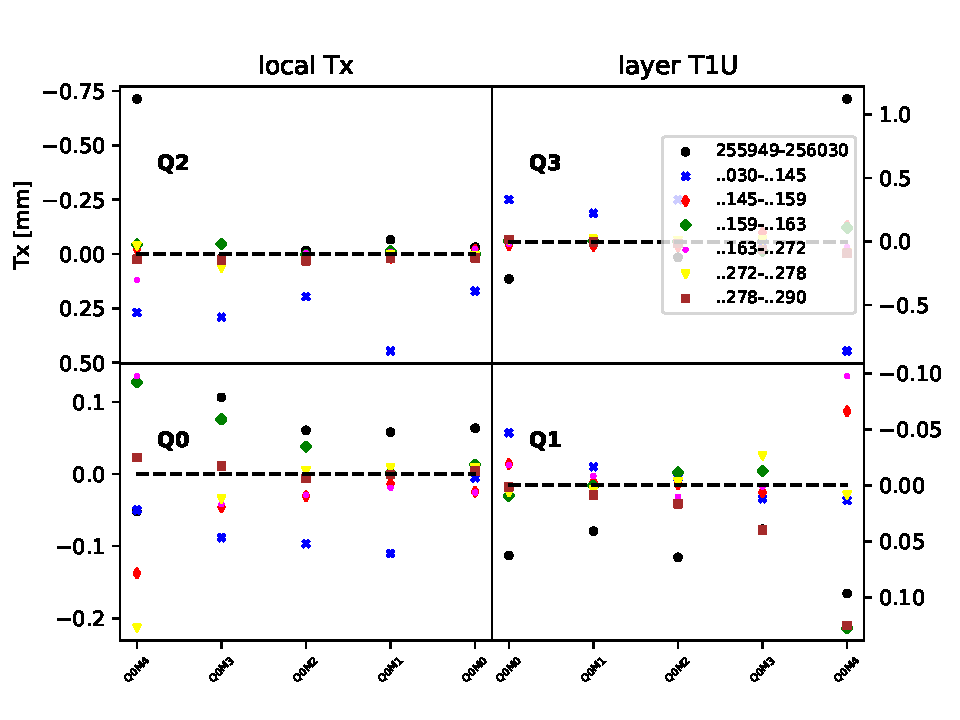
\includegraphics[width=0.9\textwidth]{plots/stability_plots/diff_data_T1U_Tx.pdf}
      \end{figure}
    \end{column}
      \begin{column}[c]{0.48\textwidth}
        \begin{figure}
          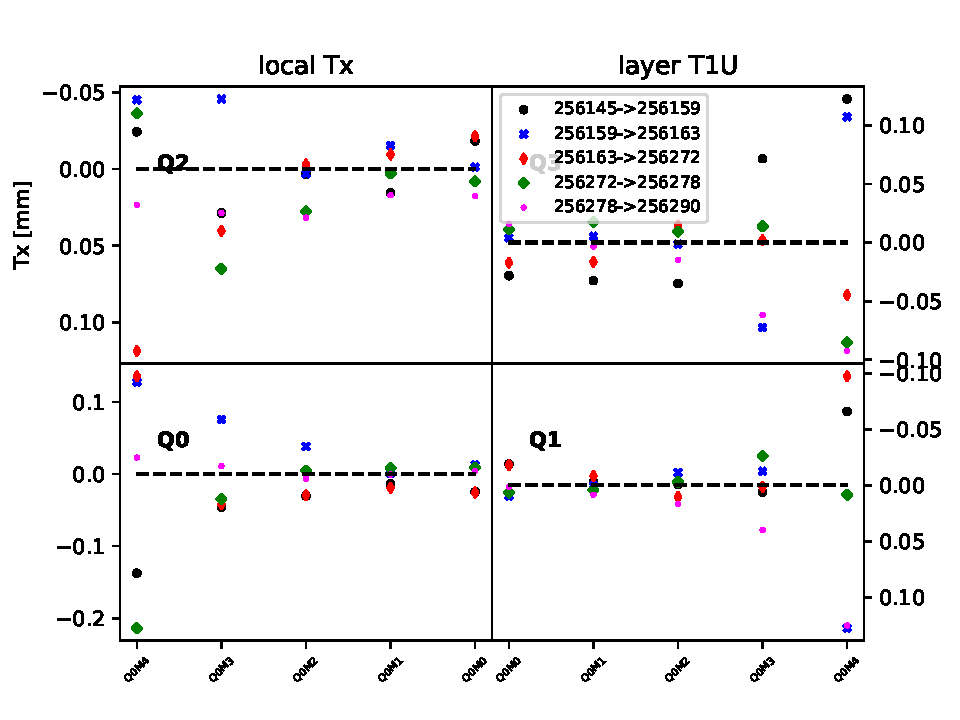
\includegraphics[width=0.7\textwidth]{plots/stability_plots/diff_reduced_Tx_T1U_Tx.pdf}
          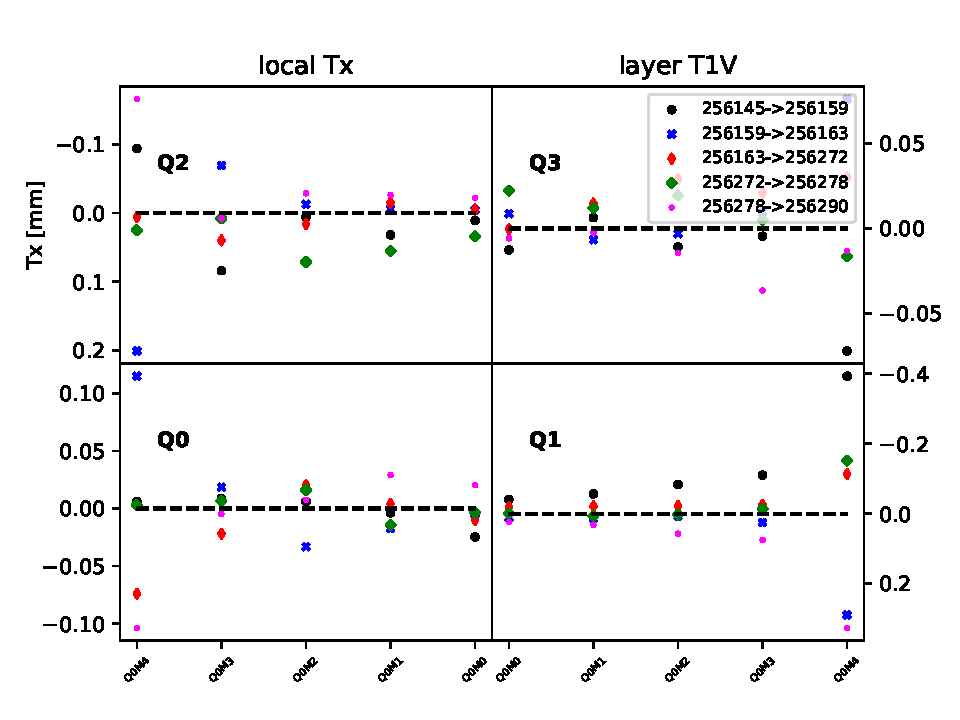
\includegraphics[width=0.7\textwidth]{plots/stability_plots/diff_reduced_Tx_T1V_Tx.pdf}
        \end{figure}
      \end{column}
  \end{columns}
\end{frame}

\begin{frame}\frametitle{Difference between runs: Tz}
  \begin{columns}
    \begin{column}[c]{0.48\textwidth}
      \begin{itemize}
        \item $\bullet$\, Tz a little worse in performance as expected
        \item $\bullet$\, similar picture as for Tx
        \item $\bullet$\, 
      \end{itemize}  
    \end{column}
    \begin{column}[c]{0.48\textwidth}
      \begin{figure}
        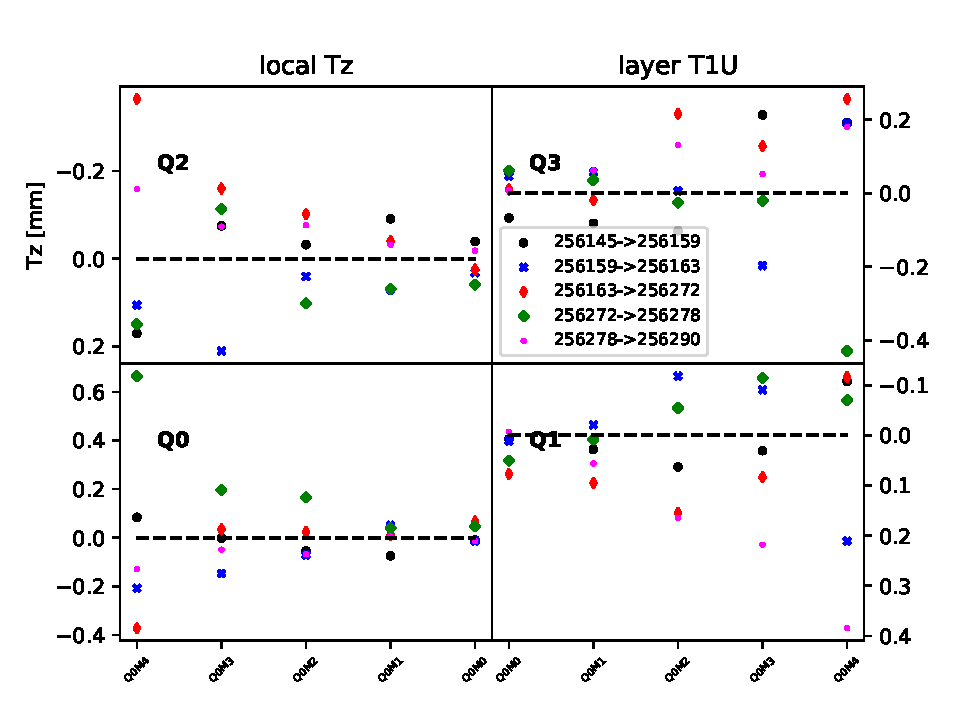
\includegraphics[width=0.7\textwidth]{plots/stability_plots/diff_reduced_Tz_T1U_Tz.pdf}
      \end{figure}
    \end{column}
  \end{columns}
\end{frame}

\begin{frame}%\frametitle{}
  \begin{columns}
    \begin{column}[c]{0.9\textwidth}
      \begin{itemize}
        \item $\bullet$\, The change in module position from run to run is a maximum of 100 $\mu m$ for the modules M0 \to M3 in Tx
        \item $\bullet$\, This is for runs from the same fill, or if there are no big changes between fills
        \item $\bullet$\, M4 moves at max 400 $\mu m$
        \item $\bullet$\, there is no visible difference between magUp and magDown polarity
      \end{itemize}  
    \end{column}
  \end{columns}
\end{frame}

\begin{frame}\frametitle{Backup}
  \begin{columns}
    % \begin{itemize}
    %   \item $\bullet$\, Module movement between runs is at most 200 $\mu m$ at the outer modules (less statistics)
    %   \item $\bullet$\, often less than 100 $\mu m$ in all other modules
    %   % \item $\bullet$\, \to we expect the modules to not move more than 100 $\mu m$ on average between runs
    % \end{itemize}
    \begin{column}[c]{0.48\textwidth}
      \begin{figure}
        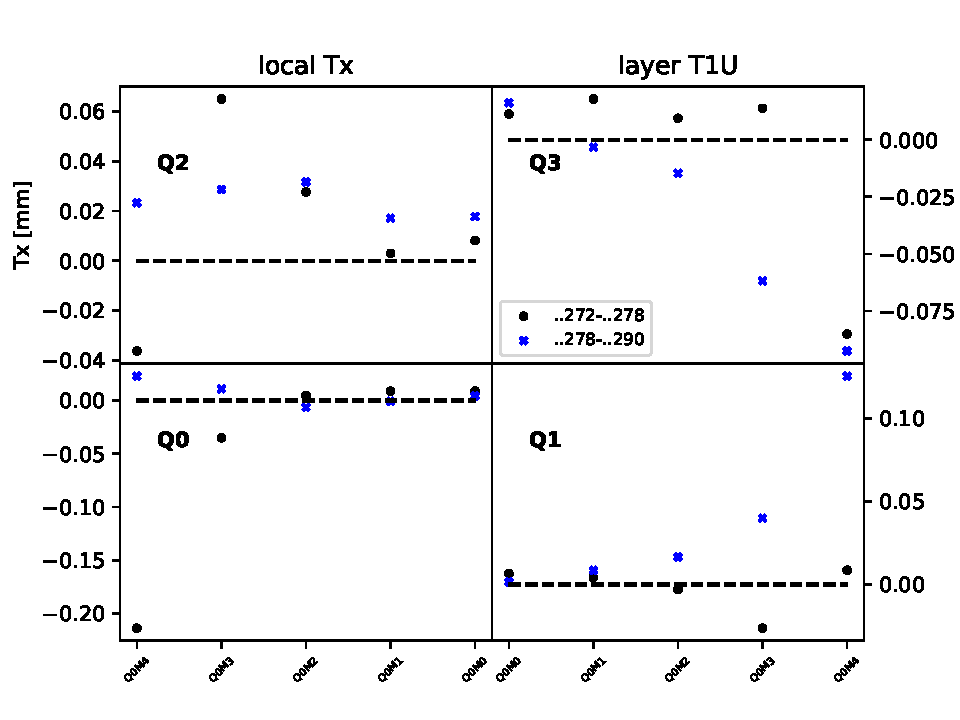
\includegraphics[width=0.9\textwidth]{plots/stability_plots/diff_MU_T1U_Tx.pdf}
      \end{figure}  
    \end{column}
    \begin{column}[c]{0.48\textwidth}
      \begin{figure}
        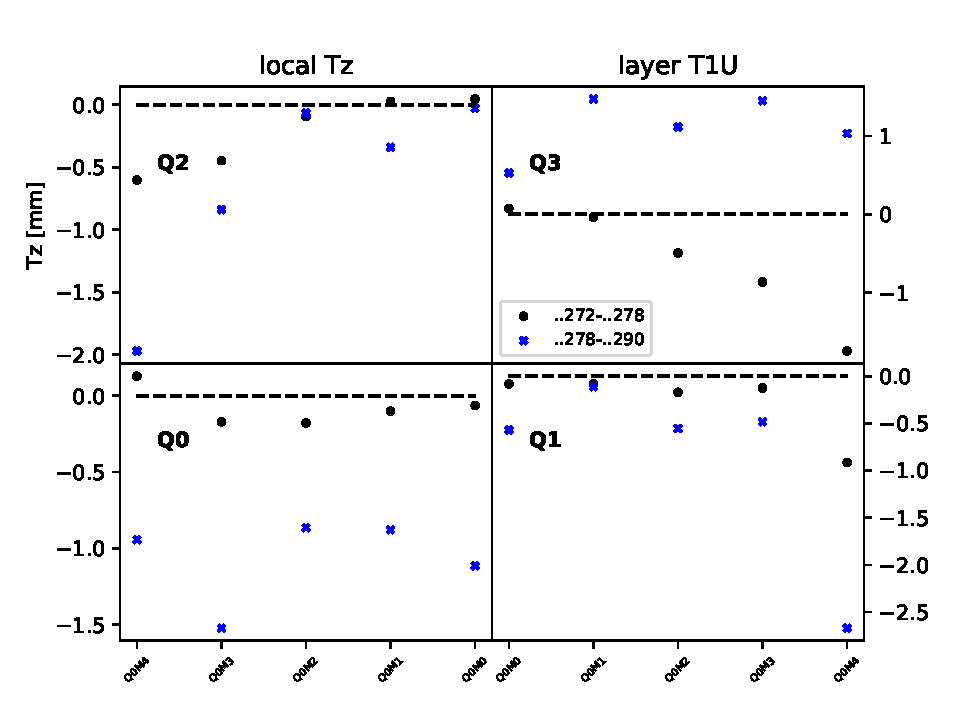
\includegraphics[width=0.9\textwidth]{plots/stability_plots/diff_MU_T1U_Tz.pdf}
      \end{figure}  
    \end{column}
  \end{columns}
\end{frame}

\begin{frame}\frametitle{Backup}
  \begin{columns}
    % \begin{itemize}
    %   \item $\bullet$\, Module movement between runs is at most 200 $\mu m$ at the outer modules (less statistics)
    %   \item $\bullet$\, often less than 100 $\mu m$ in all other modules
    %   % \item $\bullet$\, \to we expect the modules to not move more than 100 $\mu m$ on average between runs
    % \end{itemize}
    \begin{column}[c]{0.48\textwidth}
      \begin{figure}
        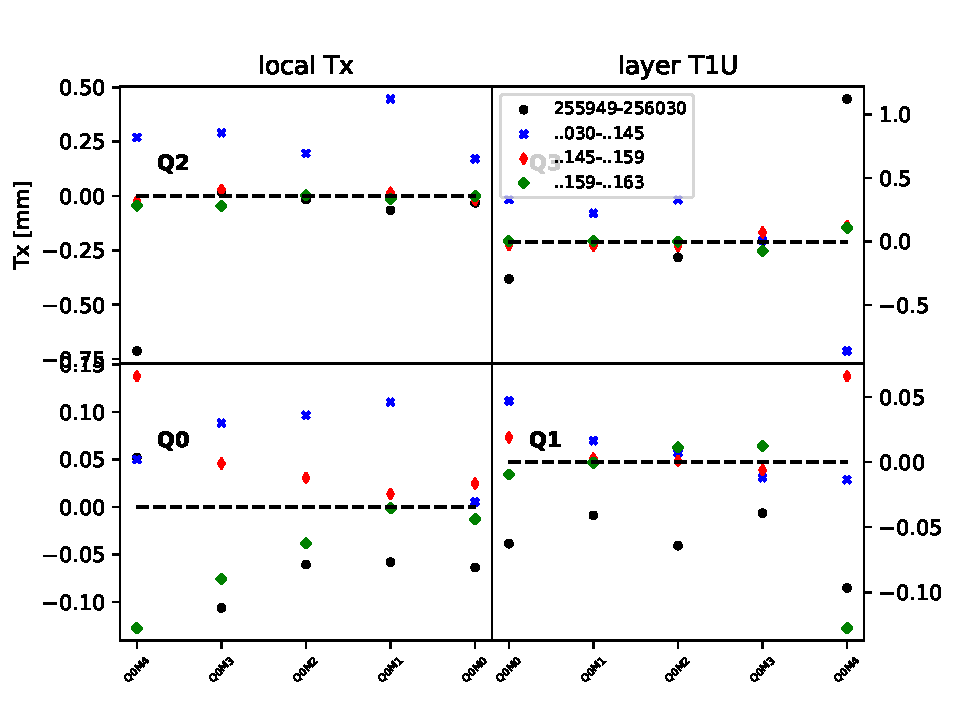
\includegraphics[width=0.9\textwidth]{plots/stability_plots/diff_MD_T1U_Tx.pdf}
      \end{figure}  
    \end{column}
      \begin{column}[c]{0.48\textwidth}
        \begin{figure}
          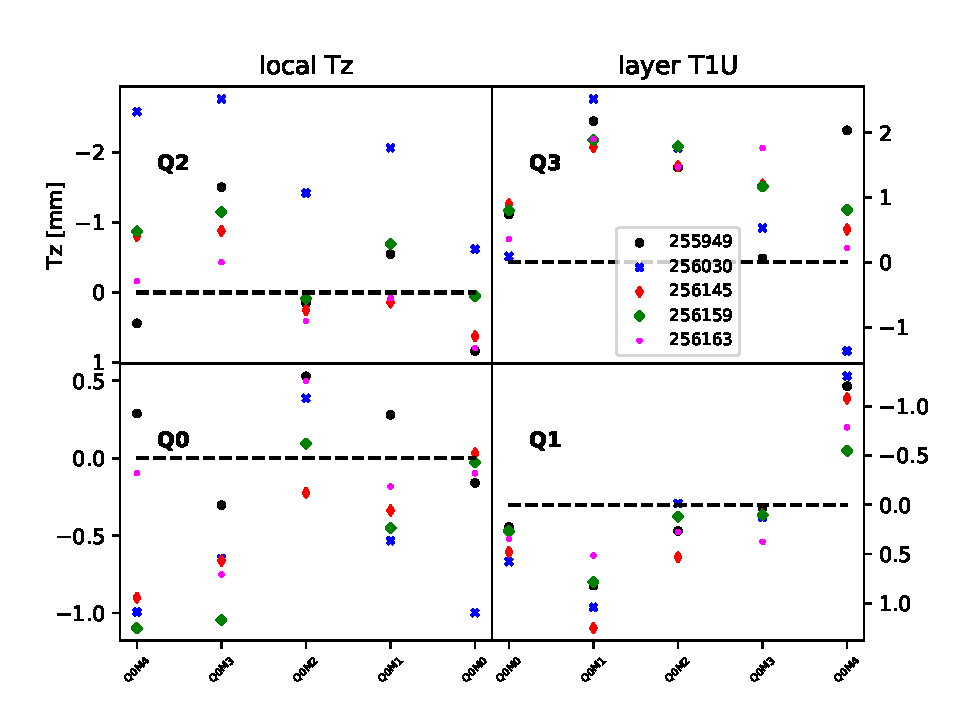
\includegraphics[width=0.9\textwidth]{plots/stability_plots/diff_MD_T1U_Tz.pdf}
        \end{figure}  
      \end{column}
  \end{columns}
\end{frame}

\end{document}
